\newpage
\section{Problema 2: Algoritmo Exacto para List Coloring}

\subsection{Descripción de la problemática}

\subsection{Resolución propuesta y justificación}

El pseudocódigo de nuestro algoritmo es el siguiente:

% \begin{algorithmic} 

% \STATE \texttt{Ordenar pasillos de mayor a menor}
% \STATE \texttt{$suma = $ metros a clausurar (inicializada en cero)}
% \FOR{\texttt{Cantidad de pasillos}}
% 	\IF {\texttt{El pasillo conecta dos conjuntos disjuntos de pasillos}}
% 		\STATE \texttt{Unir el conjunto mas chico al mas grande}
% 	\ELSE
% 		\STATE \texttt{$suma += $ la longitud del pasillo actual}
% 	\ENDIF
% \ENDFOR
% \STATE \texttt{devolver $suma$}
% \end{algorithmic} 

\subsection{Análisis de la complejidad}

\subsection{Código fuente}

% A continuación se incluyen las partes más relevantes del código.\\
% La clase \emph{Main.java} se basa en crear el grafo con la lista $ps$ y llamar a \textit{kruskal}:
% \lstinputlisting[name=pp, numbers=left, frame=lines, firstline=33, lastline=35]{../src/ej3/src/Main.java}
% Los métodos que manipulan al grafo que se encuentran en la clase \emph{Grafo.java}
% \lstinputlisting[name=gr, numbers=left, frame=lines, firstline=11, lastline=46]{../src/ej3/src/Grafo.java}
% %\newpage
% Por último la clase \emph{UnionFind.java}
% \lstinputlisting[name=uf, numbers=left, frame=lines, firstline=8, lastline=59]{../src/ej3/src/UnionFind.java}

\subsection{Experimentación}

\subsubsection{Constrastación Empírica de la complejidad}
\subsubsection{Mejor Caso}
\subsubsection{Peor caso}

% \begin{figure}[H]
% 	\centering
%  	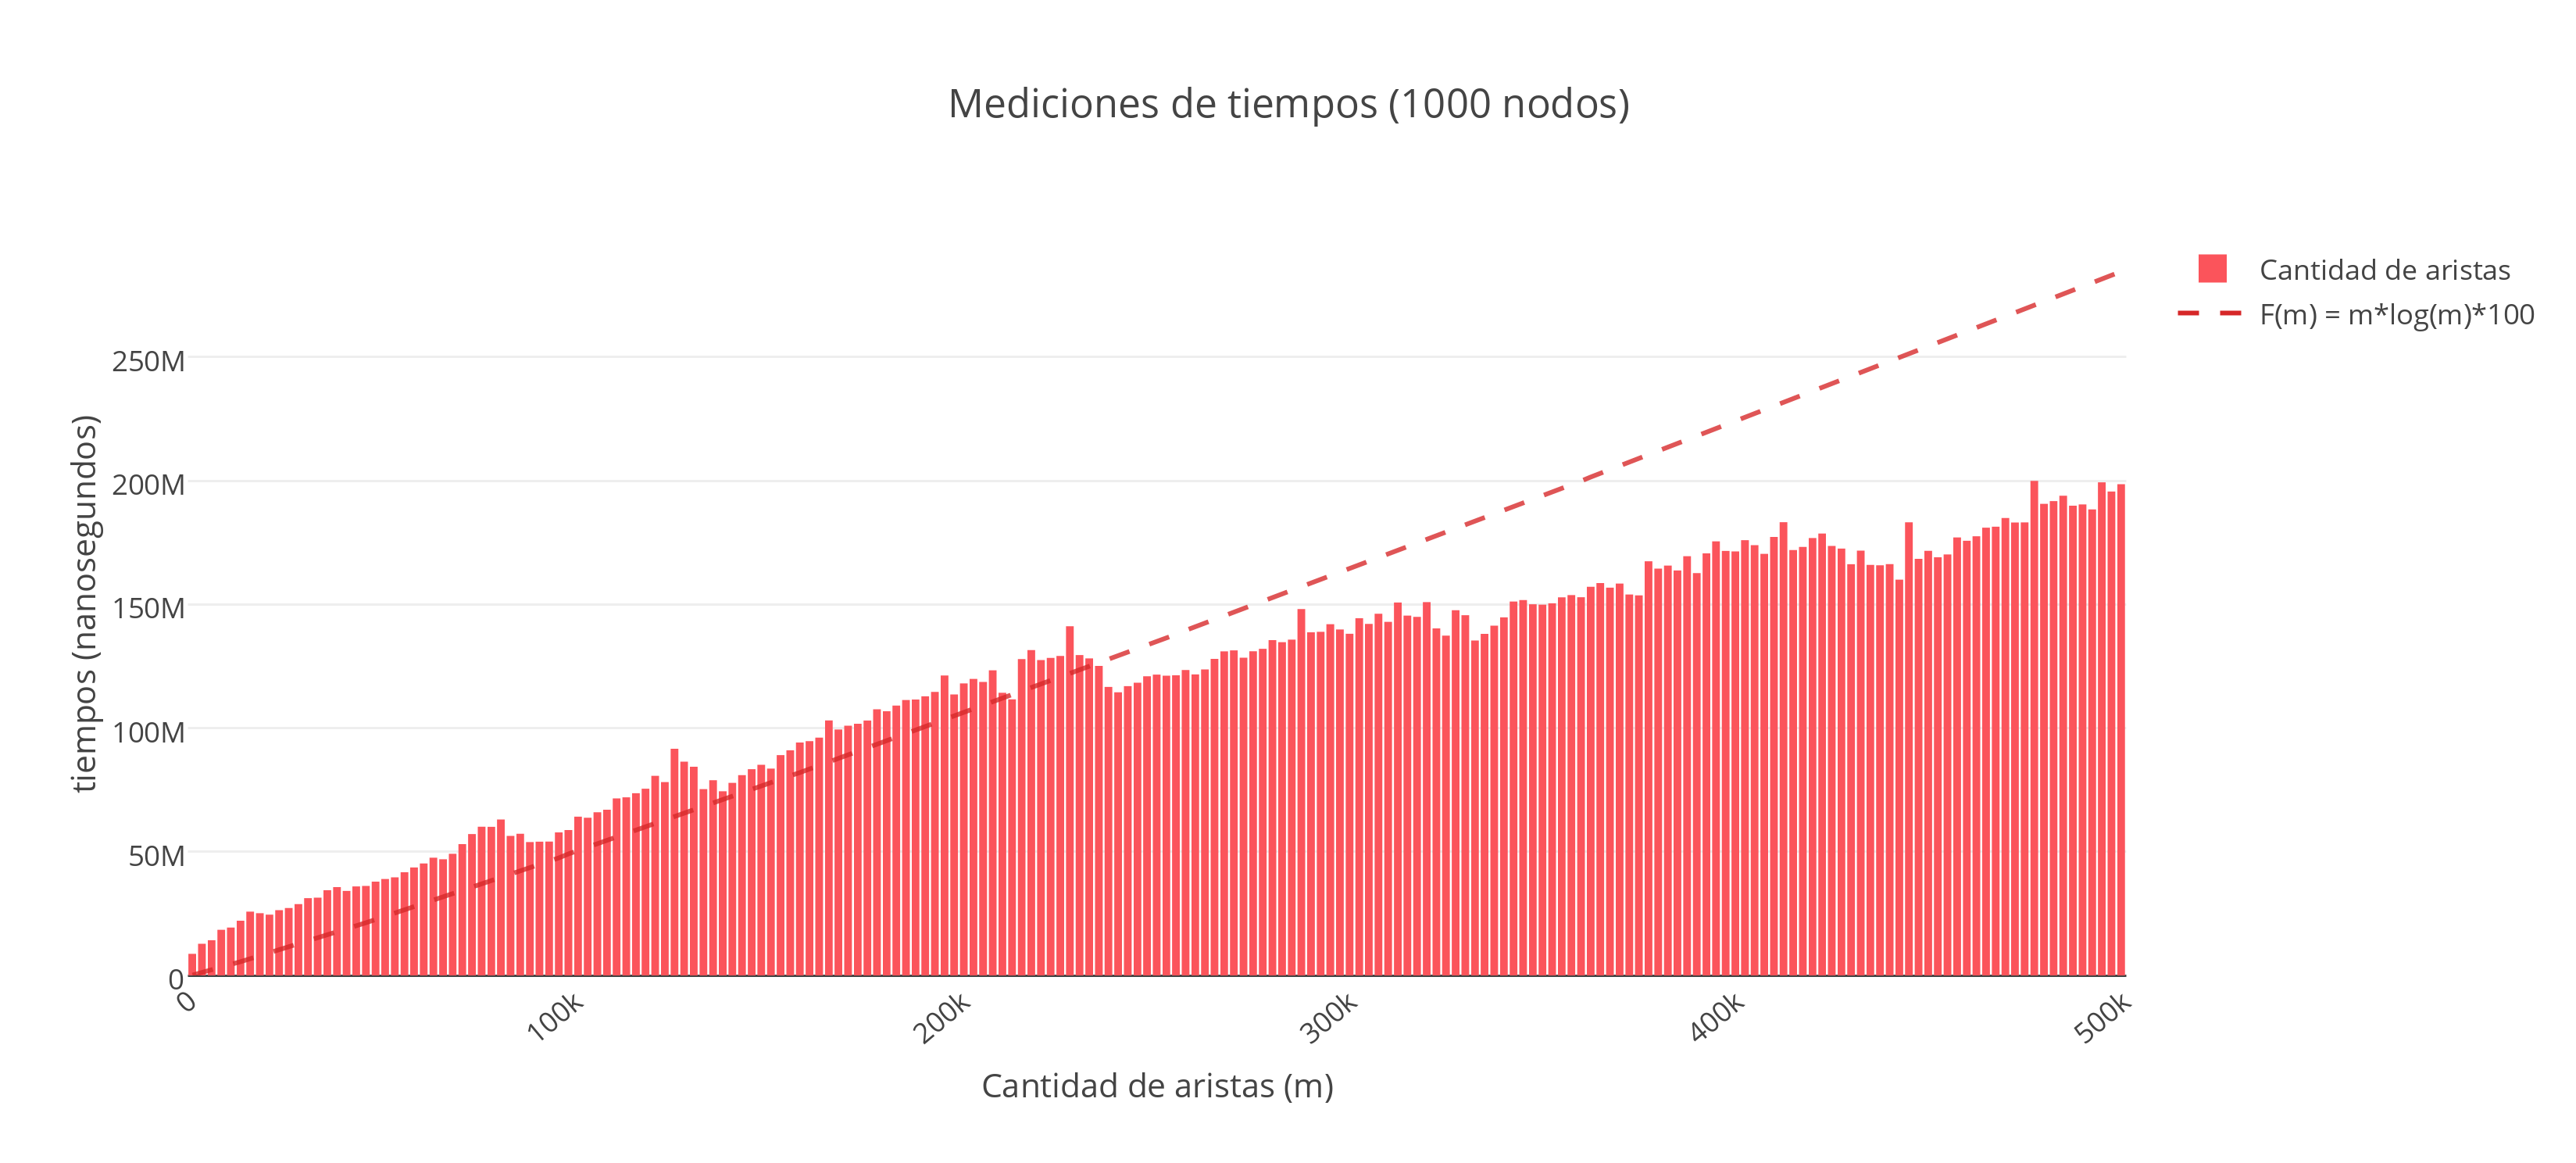
\includegraphics[scale=0.6]{imagenes/ej3/tiempos1000B.png}
% 	\caption{Medición de tiempo promedio con $n$ fijo en 1000}
% 	%\label{tiemposprom}
%  \end{figure}